%************************************************
\chapter[Experimental evaluation]{Experimental evaluation}\label{ch:Experiment}
%************************************************

\begin{flushright}{\slshape Conta ciò che si può contare, misura ciò che è misurabile e rendi misurabile ciò che non lo è.} \\ \medskip
    ---  Galileo Galilei
\end{flushright}

Usually, robotics is a prime example of applied engineering. Everything starts with a practical problem, for instance, how to autonomously navigate in a crowded environment. From that, multiple technological solutions are imagined, designed and implemented. When a solution is ready to be executed is deployed on the robot and tested. A failure results in a step back, in creating a different solution, while a success pushes the engineer to look for a new problem. 

Unfortunately, our work does not target a robotic problem, but a robotic meta-problem. How to make the process of creating technological solutions more streamlined and more accessible, in a way that failures are only minor setbacks in resolving a problem. This makes the experimental evaluation different and more challenging, since it has to include the human element.

In this chapter, we present two experimental evaluations that we used to test and asses our approaches. First, we present a robotic use case, where the architecture of an autonomous wheelchair is implemented from scratch using a model-based approach combined with automatic code generation. Then, we push the boundaries of our capabilities-based approach, by creating a web interface that developers with no experience in robot development can use to design and develop algorithms to interact with different robotic platforms.

\newpage

\minitoc
\newpage

\section{The PMK use case}
\label{sec:pmk}

\begin{figure}[t]
\centering
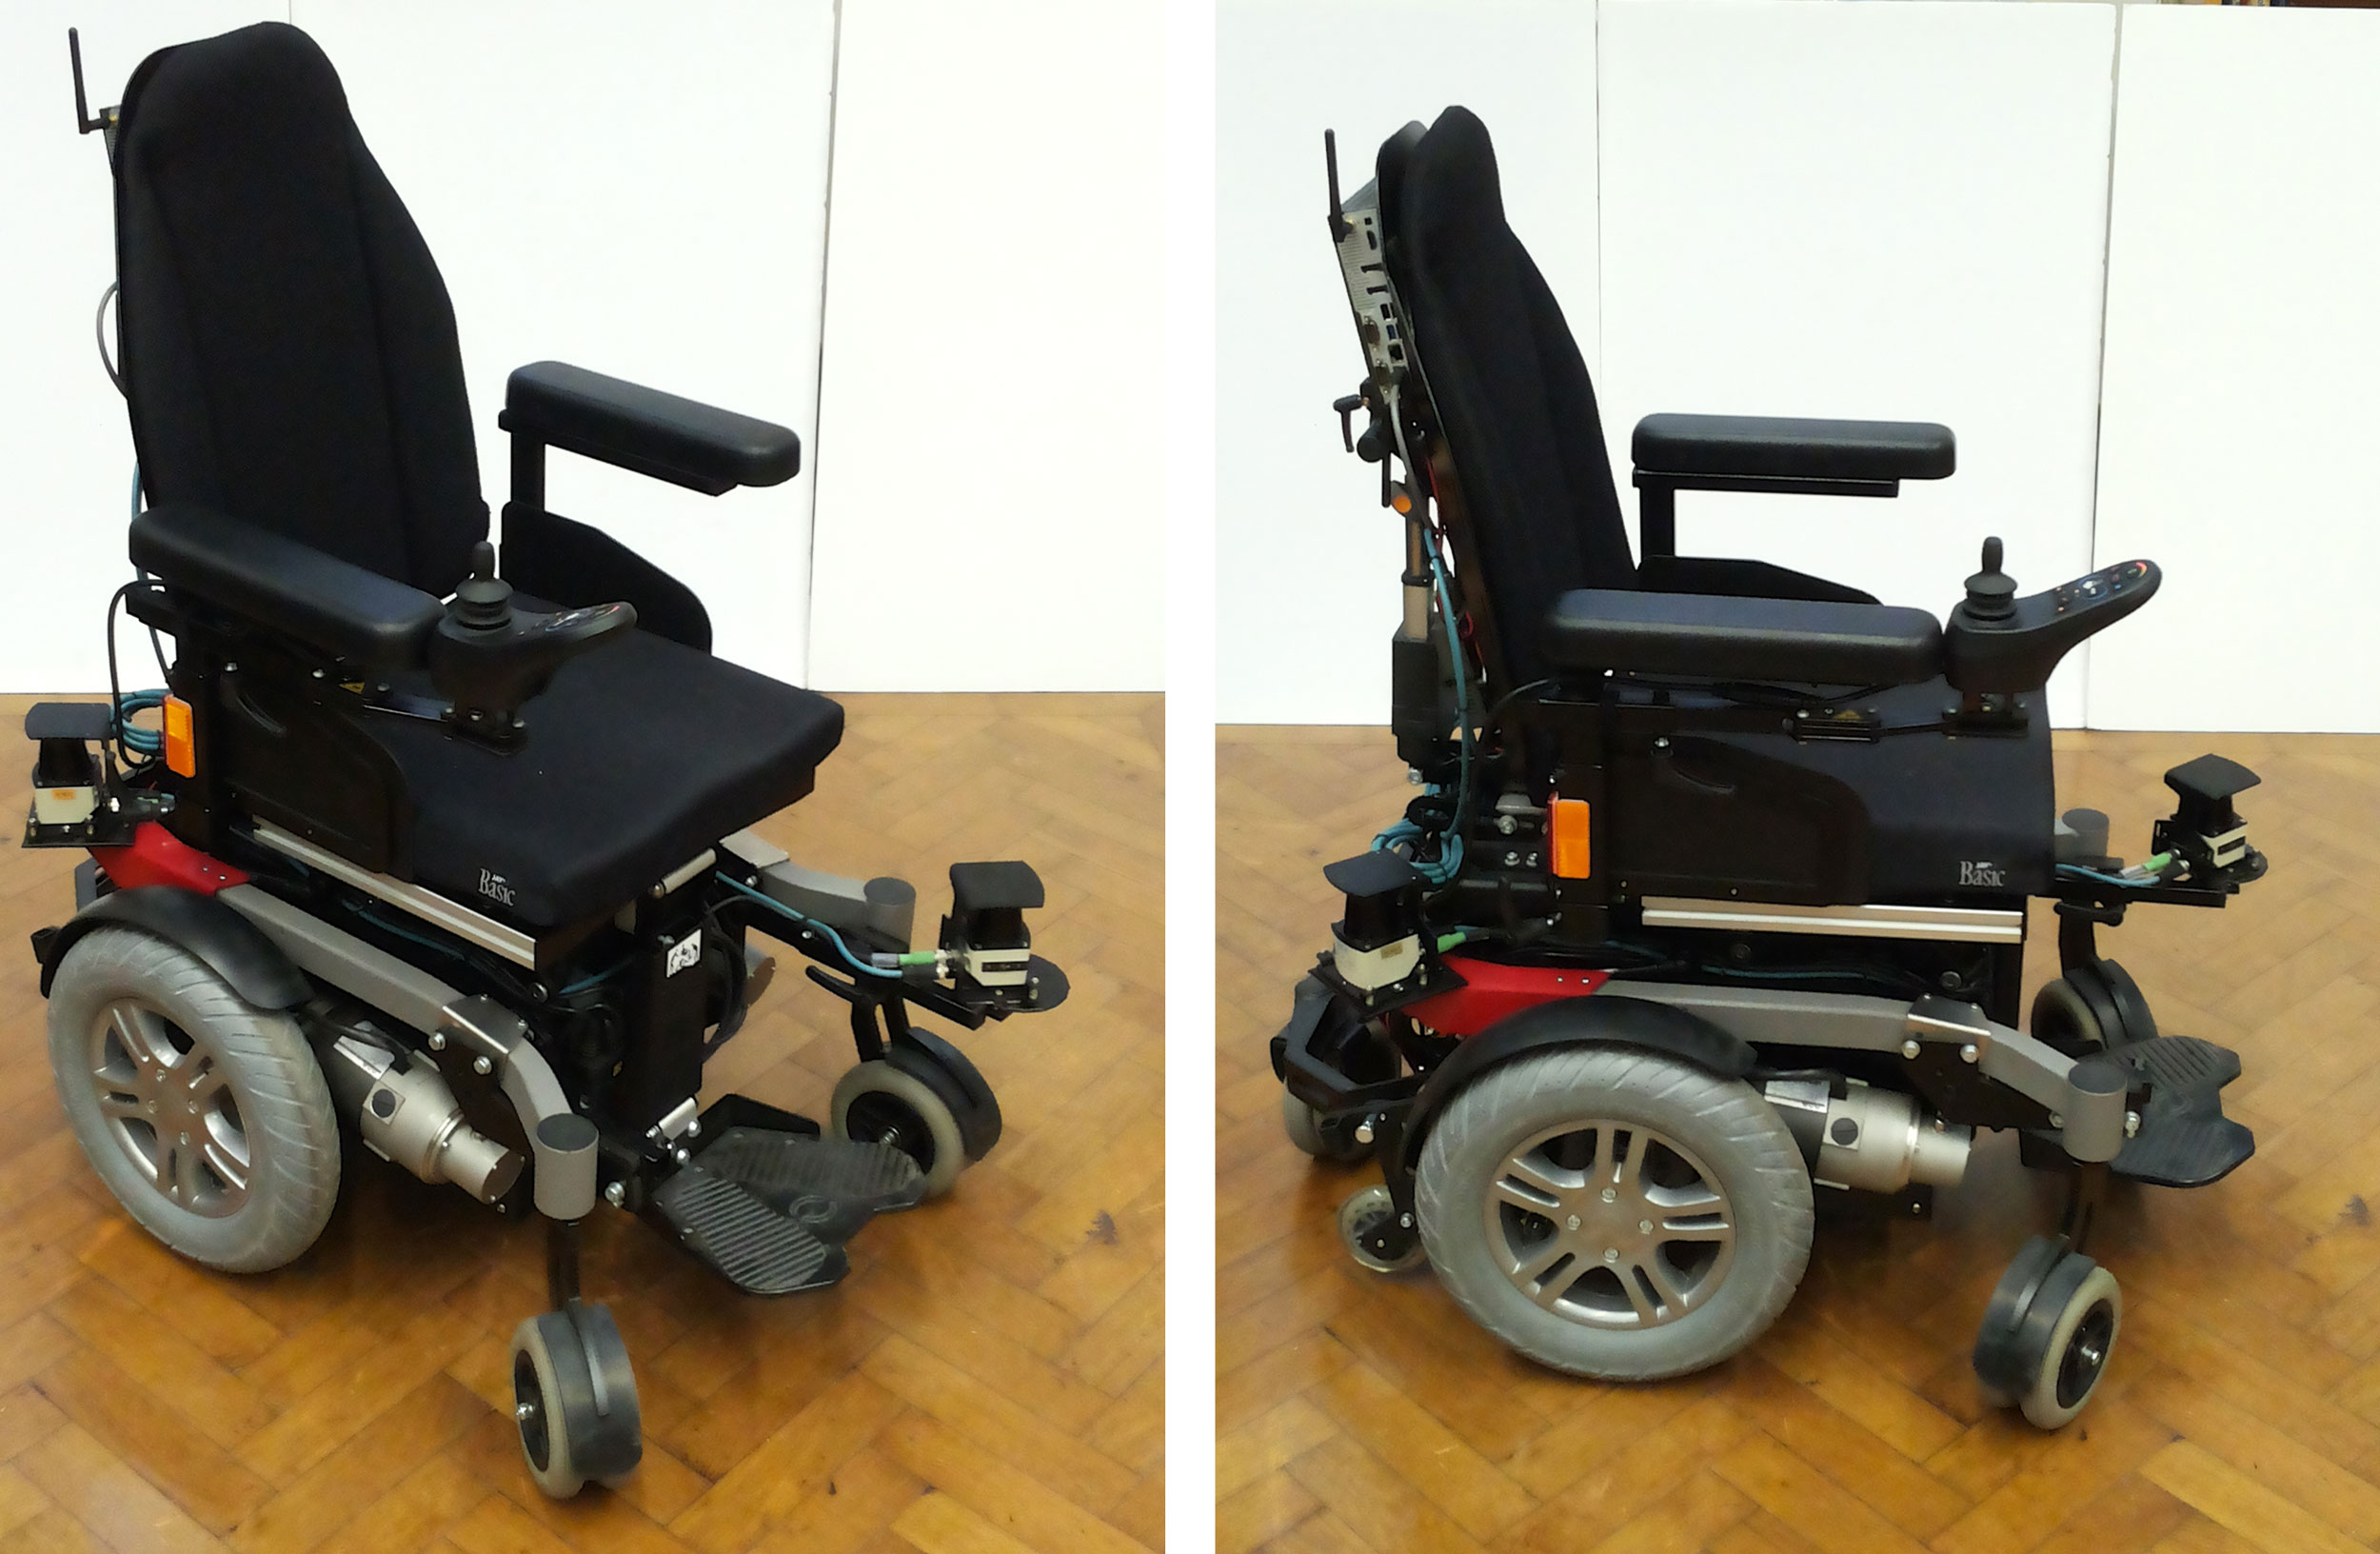
\includegraphics[width=0.95\textwidth]{gfx/pmk/pmk_plat}
\caption{The Twist T4 2x2 wheelchair modified using the Personal Mobility Kit.}
\label{fig:pmk}
\end{figure}

In this section we give a detailed description of a test use case where a model-based approach has been used to replicate and reimplement an existing architecture developed with traditional techniques. We decided to start from an already implemented and fully functional system, to show that is possible to achieve the same level of functionalities of the original application by combining a model-based design with automatic programming.

The target robot is an electric wheelchair modified to be controlled with a computer, and equipped with various sensors to achieve levels of autonomy and teleoperation. The wheelchair used as the starting platform is a commercial model (\textit{Twist T4 2x2}) produced by Degonda Rehab SA; it is suitable for both indoor and outdoor usage and it has high manoeuvrability thanks to the two-wheeled dynamics. The conversion from traditional electric wheelchair to autonomous robotic platform is achieved using the Personal Mobility Kit (PMK), which consists of four elements.
\begin{itemize}
\item Encoders connected to the electric motors controlling the wheels, which provide odometry information.
\item Two \textit{Sick TiM 561} laser scanner distance sensors, which provide a 360-degrees coverage around the wheelchair. They are used to map the environment, assist in the localisation of the robot and detect unexpected obstacles.
\item \textit{Shuttle DS81L}, an high-performance slim PC specifically designed for automotive and robotics applications. It is the on-board computer of the robot, it runs ROS and all the application code.
\item The software components necessary to achieve the assisted and autonomous functionalities.
\end{itemize}

The PMK is designed to be an add-on that is possible to mount over any existing electric wheelchair to convert it into an autonomous or semi-autonomous platform. Thus, within the architecture we will present, the only platform specific part is the interface used to communicate with with on-board electronics. Everything else is a modular design that can be adapted to various physical platforms.

A commercial electric wheelchair supports manual control through a joystick placed on one of the armrest. While this is suitable for most of users, there are cases of severe disability where the patients can only partially or cannot operate the joystick. The objective of PMK is to extend the functionalities of an electric wheelchair to provide assisted and autonomous control. In particular, the implemented software supports four different drive modes.

\paragraph{Manual with PMK off} This is the native configuration of the wheelchair. The user controls the movements directly with the on-board joystick. It is important to maintain the original operational mode even after the modification introduced by the PMK. The electric wheelchair should remain completely functional and operative even if an hardware or software malfunction causes the PMK to stop working. This acts as a fallback emergency configuration.
\paragraph{Manual with PMK on} In this configuration the PMK is active, but the user is still completely in control of the wheelchair. When mediated by the software system, the robotic platform can be controlled remotely by using a wireless joypad or directly with the on-board joystick. A priority system ensures that the input from the joystick always has precedence over teleoperation. This is the neutral configuration of PMK, when the system is active, but not performing any action. This mode is particularly useful during the set up phases of the autonomous wheelchair (\eg, environment mapping).
\paragraph{Assisted} In this mode the PMK is enabled and actively meditates the commands coming from any input device. The aim of this configuration is to help the user operate the wheelchair by avoiding obstacles. Set-points sent from the wireless joypad or on-board joystick are processed and, if necessary, modified to avoid obstacles perceived by the two on-board laser scanners. As for the previous mode, the commands coming from the joystick have the priority over the wireless joypad.
\paragraph{Autonomous} Here the wheelchair is fully autonomous, and the PMK is in charge of controlling the movements. The user can request a specific goal (\eg, ``take me to the kitchen''), then the robotic platform will automatically reach the destination avoiding any obstacle along the way. For safety reasons, it is always possible to override the commands sent by the PMK in autonomous mode using the on-board joystick.

\medskip
These are all the main functionalities of the electric wheelchair when equipped with the Personal Mobility Kit. Our aim is to create a system designed and developed using a model-based approach combined with automatic programming that exploits all the problem-related implementations already created for the original architecture and combine them with automatically generated ROS nodes, while maintaining the same functionalities.

\begin{landscape}
	\begin{figure}[t]
	\centering
	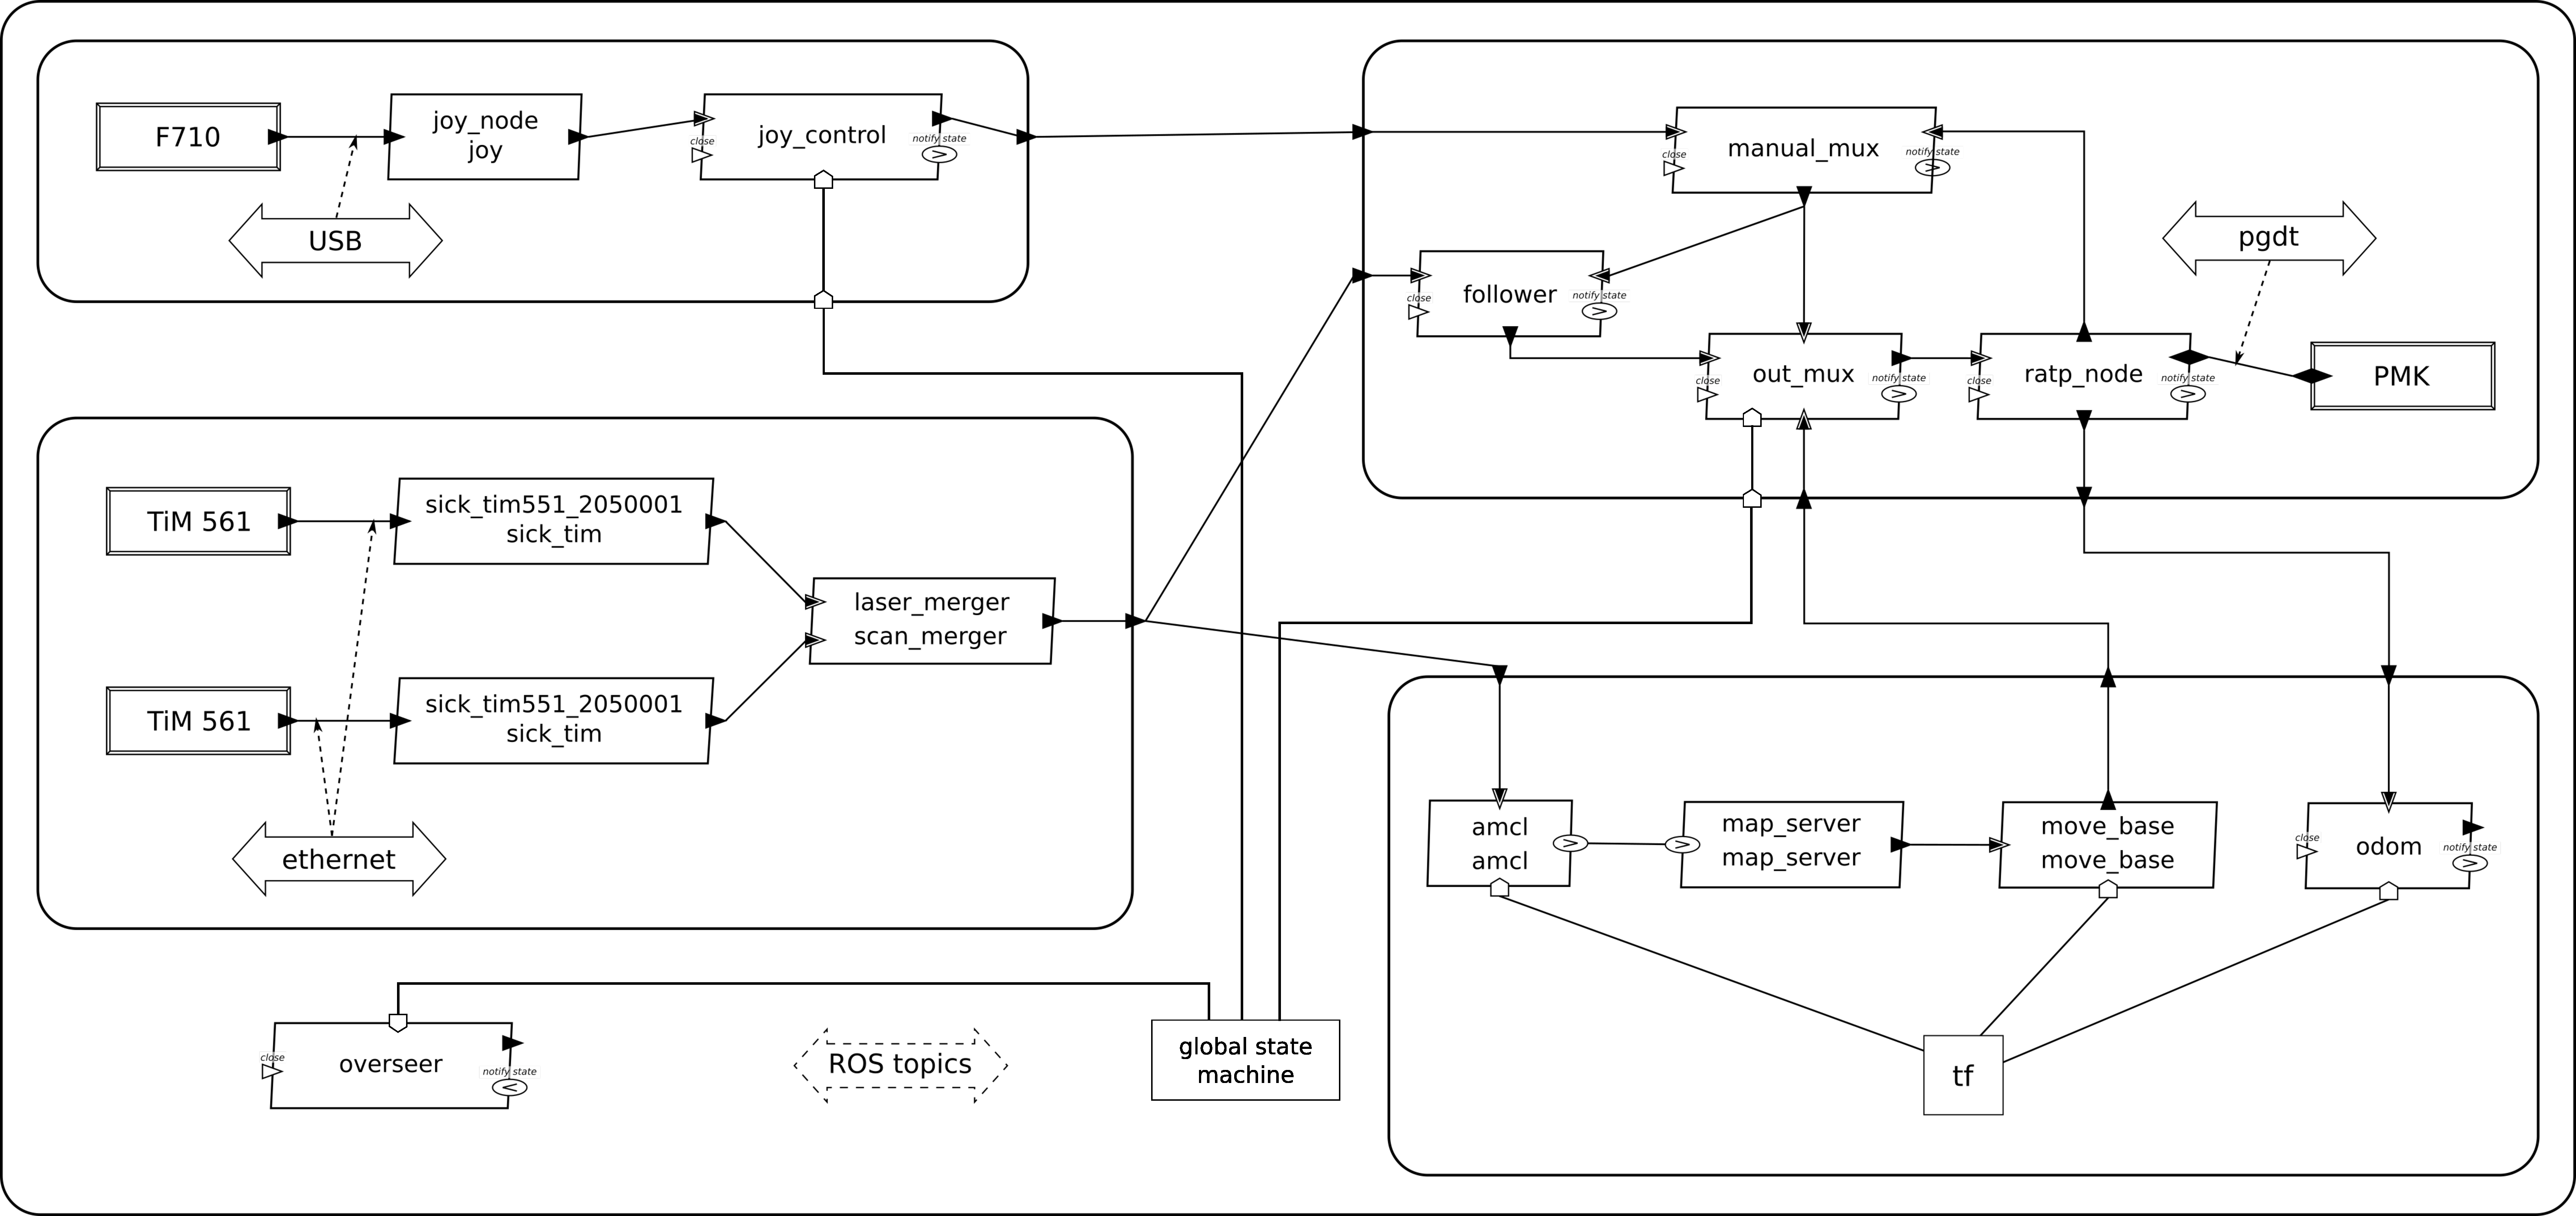
\includegraphics[width=0.95\textheight]{gfx/pmk/model}
	\caption[Graphical AADL modelling the entire autonomous wheelchair architecture.]{Graphical AADL modelling the entire autonomous wheelchair architecture. While the virtual bus representing the ROS communications is included, the binding with the topics are omitted for clarity.}
	\label{fig:pmk-model}
	\end{figure}
\end{landscape}


\subsection{Model}
\label{sec:pmk-model}
The first step of the design of an architecture is to create the model. We did so by following the definitions and meta-models introduced in Chapter~\ref{ch:Modelling}. Figure~\ref{fig:pmk-model} shows the graphical AADL modelling the architecture of the robotic wheelchair. To organise and generalise the architecture we exploited the nesting capability of AADL by creating a hierarchical structure of system of systems. Each subsystems capture a specific functionality of the robot, and they are meant to be modular parts of the design that can be replaced when necessary. For example, by going from laser scanner to cameras, or by replacing the navigation system based on \textit{move\_base} with a custom one, or by using a different electric wheelchair as platform.

\paragraph{Teleoperation} Similarly to the example presented in Section~\ref{sec:ros-arch}, this subsystem captures all the hardware and software components necessary to implement teleoperation. This specific models include an AADL device modelling the wireless joypad used to control the wheelchair: a Logitech Gamepad F710. Directly connected to it, the device driver, the existing ROS node \textit{joy\_node} from the package \textit{joy}; it reads the input from the joypad and converts it to ROS messages. The connection between the device and the driver is bound to an AADL bus modelling the physical USB interface between the joypad and the computer. The last software component in the subsystem is a node specifically designed for this application, \textit{joy\_control} is in charge of converting the messages coming from the device driver to velocity set-points to directly control the wheelchair (\ie, from \textit{Joy} to \textit{Twist} messages). Additionally, this node controls the global state machine of the system that selects the current driving mode (\ie, one of the four presented in Section~\ref{sec:pmk}).

Given the criticality of this step, the communication does not happen through ROS topics or services, but by using a shared memory area. To capture this behaviour in the model we use a require data access port on the process modelling \textit{joy\_control}. On its frontier, the system exposes an outgoing port associated with the velocity command to relay the set-points generated by the teleoperation subsystem to the rest of the architecture. Moreover it has a data access to bridge the connection coming from the driving mode selection node (\ie, \textit{joy\_control}) to the shared memory area hosting the global state machine. Encapsulating the model in a system increases the modularity of the design, since it defines exactly the expected interfaces of the subsystem and makes it replaceable with a similar configuration (\eg, a different physical input) without altering the entire architecture.

\paragraph{Sensing} For the navigation and obstacle avoidance to work correctly, they need a single measurement from the laser rangefinder. Since the robotic platform is equipped with two sensors, the aim of the sensing subsystem is to unify their measurements in a single output. For this reason only one outgoing port is present on the system frontier representing the merged scan topic. Here there is a clear example on how multiple instances of same element can coexist as subcomponents. There are two occurrences of the same AADL device modelling the physical sensors mounted on the wheelchair, consequentially, the device driver component is duplicated too. As for the teleoperation subsystem, the connection between each laser scanner and the corresponding driver is bound to a model of a physical bus; but since the communication goes through an Ethernet connection it is a different component. All the connections converge in a single node in charge of merging the measurements coming from each laser rangefinder, that are then relayed outside the subsystem through the output port present on the frontier. In this system there is no custom node, since all of them come from existing packages or legacy implementations.

\paragraph{Navigation} This subsystem mostly contains legacy nodes from ROS Navigation. A node implementing adaptive Monte Carlo localisation to estimate the position of the robot in a known environment (\textit{amcl}), a node to store and share the current map of the environment (\textit{map\_server}), and the main navigation node (\textit{move\_base}) implementing global planning on the known map and local planning on the map generated in real time. To work, ROS Navigation requires laser measurements and odometry information, the former comes from the sensing subsystem, while the latter is generated by the custom \textit{odom} node included in the navigation subsystem; it receives the current speed from the wheelchair and uses it to estimate the position of the platform. The odometry node supports two types of output, as visible from the features of the AADL process: an \textit{Odometry} message, published on a topic and modelled using an output port, and \textit{tf}, modelled thorough a data access directly connected to the data component representing the centralised collection of all the reference frames. Since \textit{tf} is the backbone of ROS Navigation, and it is used only by nodes in this subsystem, it was reasonable to model the data component representing \textit{tf} here. Differently from the two previous subsystems (\ie, teleoperation and sensing), here there is no need to model any physical bus since this is a pure software system. The frontier of the navigation subsystem is more complex, since it has an input port for the laser measurements, another input port for the speed of the wheelchair and  an output port for the set-point generated by \textit{move\_base}. Abstracting the structure and interface of the navigation subsystem is particularly important because it is the part of the architecture that is often subject to changes. It is common to use the same platform to test different algorithms and architectural solutions for navigation.

\paragraph{Platform} All the hardware and software components related to the physical platform are contained in this subsystem. Since they are all platform-related, each node is a custom design created specifically for this architecture. There are two hardware components: a device to model the interface between the architecture and the on-board electronics manufactured by Penny\&Giles Drive Technologies Ltd. (PGDT), and the bus representing the special hardware connection used to exchange wheelchair-specific messages. This bus and the corresponding custom device driver (\textit{ratp\_node}) act as a bridge between platform-specific data streams and ROS messages. Given the multiple driving modes of the robot where two manual inputs, potentially mediated by the system and with different priorities, coexists, together with an autonomous mode, the architecture uses a combination of two multiplexers. One is used to select the specific manual input (\ie, \textit{manual\_mux}), while the other (\ie, \textit{out\_mux}) differentiate between the different driving modes (\ie, manual, assisted and autonomous). The two multiplexers have different behaviours, \textit{manual\_mux} is based on priorities, the input coming from the on-board joystick will always override the wireless joypad, while \textit{out\_mux} changes the output depending on the current mode of the system. For this reason \textit{out\_mux} has a data access connected to the shared memory area hosting the global state machine. Finally, the last component is a node implementing local obstacle avoidance for assisted driving. Even with its peculiar configuration, the whole subsystem is designed with a general frontier, it exposes two inbound ports for the velocity commands (\ie, joypad and autonomous set-points) and one for scan messages (\ie, measurements for obstacle avoidance). The output port relays the current velocity of the wheelchair from the custom device driver node to the navigation subsystem. Additionally, as for the teleoperation subsystem, the platform system has a data access on its frontier to connect to the global state machine. By encapsulating the platform in a system, it is possible to replace it with a different wheelchair, or even with a completely different robotic platform.

\begin{figure}[t]
\centering
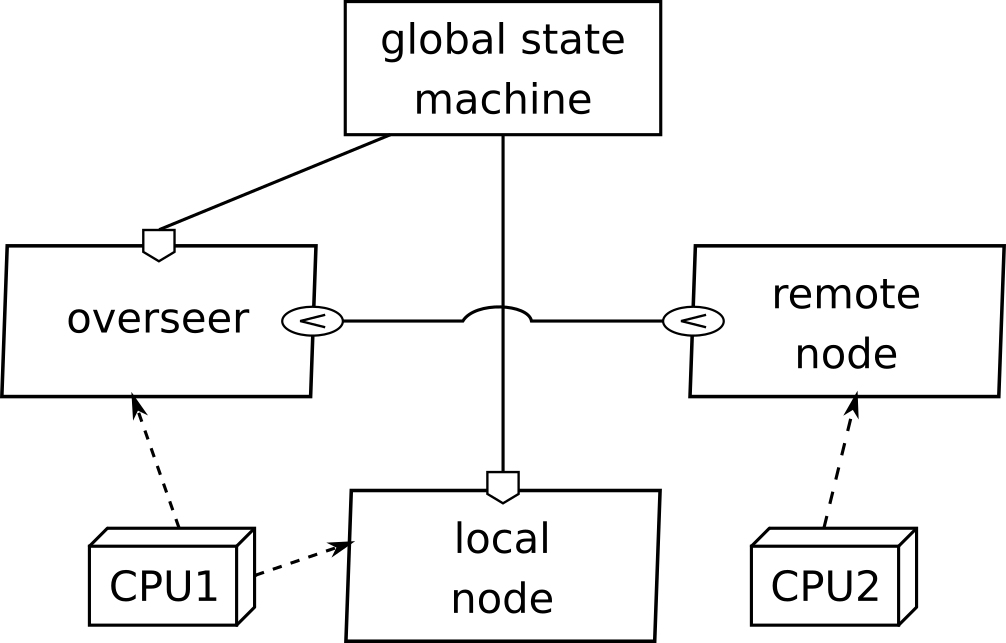
\includegraphics[width=0.7\textwidth]{gfx/pmk/overseer}
\caption{Graphical representation showing how a local and a remote node interact with the global state machine.}
\label{fig:pmk-gsm}
\end{figure}

\paragraph{Main system} To increase clarity and use the model to evoke the modularity of the architecture, we modelled it with different subsystems. However, in AADL it is necessary to define a root system to encapsulate everything, moreover, some part of the architecture are too general to be fitted in a specific subsystem. For this architecture, three components fall in this category: the \textit{ROS communication} virtual bus, the \textit{overseer} node and the global state machine. In the same way as physical buses are used in the teleoperation and platform subsystems, the \textit{ROS communication} virtual bus bindings are necessary to identify which connections model ROS communication protocols (\ie, topics or services). As originally introduced in Section~\ref{sec:ros-in-aadl} and, later, detailed in Section~\ref{sec:ros-node}, the engineered nodes are designed with a strict life cycle, and they natively support a notification system to monitor the evolution of their state. The \textit{overseer} node is in charge of collecting all the notification coming from the custom nodes, moreover it has a list of all the critical nodes (\ie, nodes that are subject to a liveness check) and trigger a transition on the global state machine if one of them stops working. The last element is the data component representing the shared memory area containing the global state machine. In the implementation, the global state machine is instantiated by the \textit{overseer}. While all the nodes in the architecture can read or modify the current state by accessing the shared memory directly, it is also possible to interact with the global state machine through a ROS service interface mediated by the \textit{overseer} (see Figure~\ref{fig:pmk-gsm}). The different approach used can be encoded in the model (\ie, connected through a data access or a subprogram call), however, in the implementation, it is determined at deployment time. In practice if the node runs on the same physical machine of the global state machine, then a shared memory approach is used, otherwise the interaction happens using ROS. 

\subsection{Automatic code generation}
In the previous section, we gave an overview of the model of the architecture by describing in details the subsystems and which functionalities they evoke. While the graphical representation of Figure~\ref{fig:pmk-model} provides a general understanding of the topology of the architecture and gives some insights on the nature of the components, it does not capture all the details necessary to correctly perform automatic code generation. First of all, nodes belong to three main categories:
\begin{enumerate*}[label=(\roman*)]
\item already implemented nodes, they are legacy nodes previously developed, they may come from the standard ROS repositories (\eg, \textit{move\_base}) or be part of the original architecture (\eg, \textit{laser\_merger}), 
\item custom nodes, they are completely modelled and will be automatically generated (\eg, \textit{odom}), 
\item special custom nodes, they are modelled correctly, but they contain unique implementation patterns that are not supported by the code generator (\eg, \textit{ratp\_node}).
\end{enumerate*} This last category will be covered in details in Section~\ref{sec:special-node}. 

As discussed in Section~\ref{sec:ros-arch}, managing existing nodes in the architecture model is extremely important, since they are an invaluable resource provided by the ROS community. During the automatic code generation, existing nodes are ignored, since they do not provide any internal implementation but are described only as interfaces. However, they are correctly included in the generation of launch files describing the current configuration of the system. Moreover, connections between components can be specialised using properties to exploit topic remapping and define the runtime name of each topic, including those of already implemented nodes. Currently, the code generator does not support the use of neither ASN.1 nor JSON schema to define the parameters of the legacy nodes. However,  it is possible to use properties to specify a standard ROS YAML file to be automatically included in the launch file as the parameter configuration of a specific node.

To automatically generate custom nodes that are compilation-ready, it is necessary to specify a series of properties. On a basic level, the designer can tune the behaviour of publisher and subscriber by setting the frequency, the queue size or the default name of the topic. Moving to a domain-specific point of view, the developer has to provide the implementations of the nodes; for this reason we decided to base our test use case on an existing architecture to exploit already implemented problem-specific code for the automatic programming phase. To understand how the process works in practice, let us take the example of the \textit{follower} node. Without considering the domain-specific implementation, this component evokes a combination of a \textit{sink} behaviour, the subscriber receiving the messages from the laser rangefinder, and a \textit{filter} behaviour, manual set-points are received, modified according to the scan measurements, eventually modified and published. This configuration is translated to the code generator to two subscribers (\ie, one for the laser and one for the input commands) and one publisher (\ie, the output set-point). Moreover, by parsing the JSON files specified as properties in the component definition, the code generator can create the internal state of the node and set default and initial values for parameters and variables. After generating all the necessary source files, it is possible to include the domain-specific implementation as an external library, defined again in properties of threads and subprograms; this is done by carefully generating all the build files that bind together the auto-generated node skeleton and the manually implemented problem-specific code. When all the file related to the node are fully generated (\ie, core node implementation, internal state, external libraries, and build configurations), it is time to create the launch files. Since the \textit{follower} node is part of the platform subsystem, it will be included in the platform-specific launch file. Here the runtime configuration of the node is generated from the JSON files and included. Moreover, as for the legacy nodes, the topics name are remapped according to the properties defined on the connections in the model. At this point, the generation of the node is complete and it is ready to be compiled and run.

\begin{figure}[t]
\centering
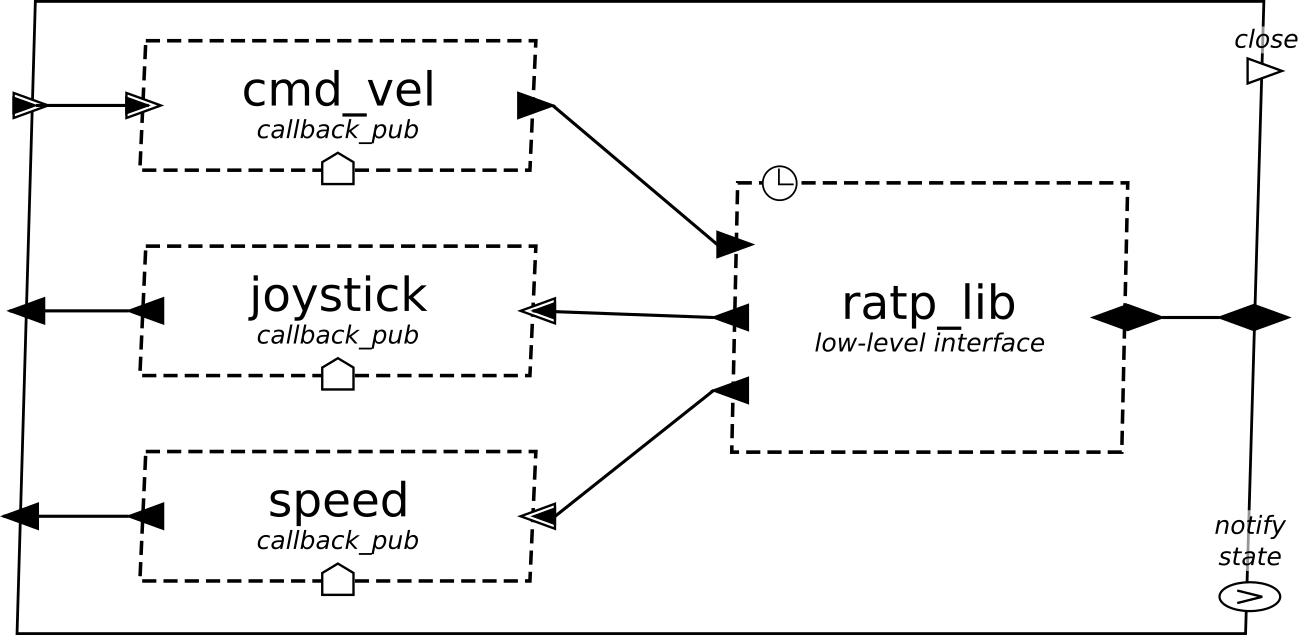
\includegraphics[width=0.95\textwidth]{gfx/pmk/ratp}
\caption[Simplified graphical representation of the AADL description modelling the ratp\_node]{Simplified (\ie, focusing only on custom defined thread) graphical representation of the AADL description modelling the ratp\_node}
\label{fig:pmk-ratp}
\end{figure}

\subsection{Special nodes}
\label{sec:special-node}
Since all the problem-specific logic was already implemented in the original architecture, every element of the new system is generated using the automatic programming approach. There is only one exception: the \textit{ratp\_node}; this node is the device driver connecting the low-level electronics of the wheelchair to the ROS-based architecture. It implements a unique interface between ROS messages and custom data streams defined by the PGDT bus, therefore it is very challenging to automatically generate the source code using an automatic programming approach. Since this node is an hybrid between a ROS-based (\ie, receiving set-points and publishing the current speed and status) and an hardware-specific (\ie, interfacing with the PMK) implementation, we can partially exploit the code generator to define a node skeleton to be refined by the developer. There are two key challenges when using this approach: first, to have a model expressive enough to capture the peculiar design of the component, and second, to generate a node in such a way that the hardware-specific functionalities can be integrated without major modifications.

To tackle the first challenge we can exploit the expressive power provided by AADL. When not extending our base templates (see Section~\ref{sec:template}) used to identify ROS elements,  AADL connections, ports and threads can be used to model any kind of communication protocol or execution flow. Figure~\ref{fig:pmk-ratp} shows a simplified (recurring elements of the base ROS node are omitted) graphical representation of the model of the \textit{ratp\_node}. It is possible to use a periodic AADL thread together with a bidirectional port on its frontier to model the communication between the component and the low-level hardware. Additional ports model the exchange from a problem-specific implementation to the ROS communication protocols.  The \textit{ratp\_lib} thread produces two outputs that are converted to ROS messages: one is the current set-point provided by the on-board joystick, and the other is the current speed of the wheelchair. Moreover, it receives one input from the rest of the system that is then converted to a format compatible with the low-level hardware: the set-point of the current active input. These port on the frontier of the low-level communication thread are connected using internal connections to the corresponding threads modelling the publishers and subscribers. However, there is a significant distinction between this model and how ROS thread are usually modelled. Threads behaving as subscribers are not triggered by a message coming from outside the component, but directly by the \textit{ratp\_lib} thread, moreover, the publisher thread output does not relay its message to the rest of the architecture, but the output port is connected directly to the low-level communication thread.

The second challenge is implicitly solved by the design of the engineered node and also by how unknown subcomponents are managed by the code generator.  As explained in Section~\ref{sec:xml-cpp}, the code generator parses a process model and implements it as a ROS node, only if it extends the base ROS node model, Moreover, among the threads defined as subcomponents, those that do not extend one of the predefined functionalities (\ie, publisher, subscriber, subscriber with publisher or service) are ignored and not processed by the automatic programming system. In the case of the \textit{ratp\_node} it means that the code generator recognises the component as a ROS node and generates all the basic structure. Additionally, the three thread modelled as ROS elements (\ie, \textit{cmd\_vel}, \textit{joystick} and \textit{speed}) but connected to the \textit{ratp\_lib} thread are correctly generated as ROS subscribers or publishers. In summary, given the model presented in Figure~\ref{fig:pmk-ratp}, the resulting generated node extends the engineered node and correctly implements the life cycle, the asynchronous spinner, the encapsulated internal state and the separation between the middleware and the problem-specific code. Moreover it contains three publishers and three subscribers. Out of these six ROS functionalities, three are already correctly implemented: the publisher for the current speed and the current command of the on-board joystick, and the subscriber for the external set-point. The other three needs to be converted from a ROS-based design to an implementation compatible with the low-level interface. While this approach may appear as an over-complication, it actually streamlines the work of the developer. The code generator handles all the ROS-related boilerplate automatically, while defining a structure that can be easily exploited; the developer only needs to focus on implementing the thread interfacing with the low-level hardware. In our implementation, we use the already created structure as a reference and replaced the callback structure of ROS with standard bindings. Basically, from the point of view of the node, the interaction still happens through a system of callbacks, however, they are not triggered by ROS, but controlled by the \textit{ratp\_thread}. 

In conclusion, while this node requires a direct intervention of the developer to modify its structure, it is more efficient to model it, generate the code to obtain a partially implemented component and then manually insert some modifications, instead of implementing it from scratch. This is possible because of the modularity and flexibility of the engineered node, and because ROS is still the main element of the component design. While our code generator currently cannot completely and successfully process this type of nodes, this mixed approach (\ie, code generation combined with heavy human intervention) gives us an insight on how future nodes with the same characteristics could be automatically generated.


\begin{landscape}
	\begin{figure}[t]
	\centering
	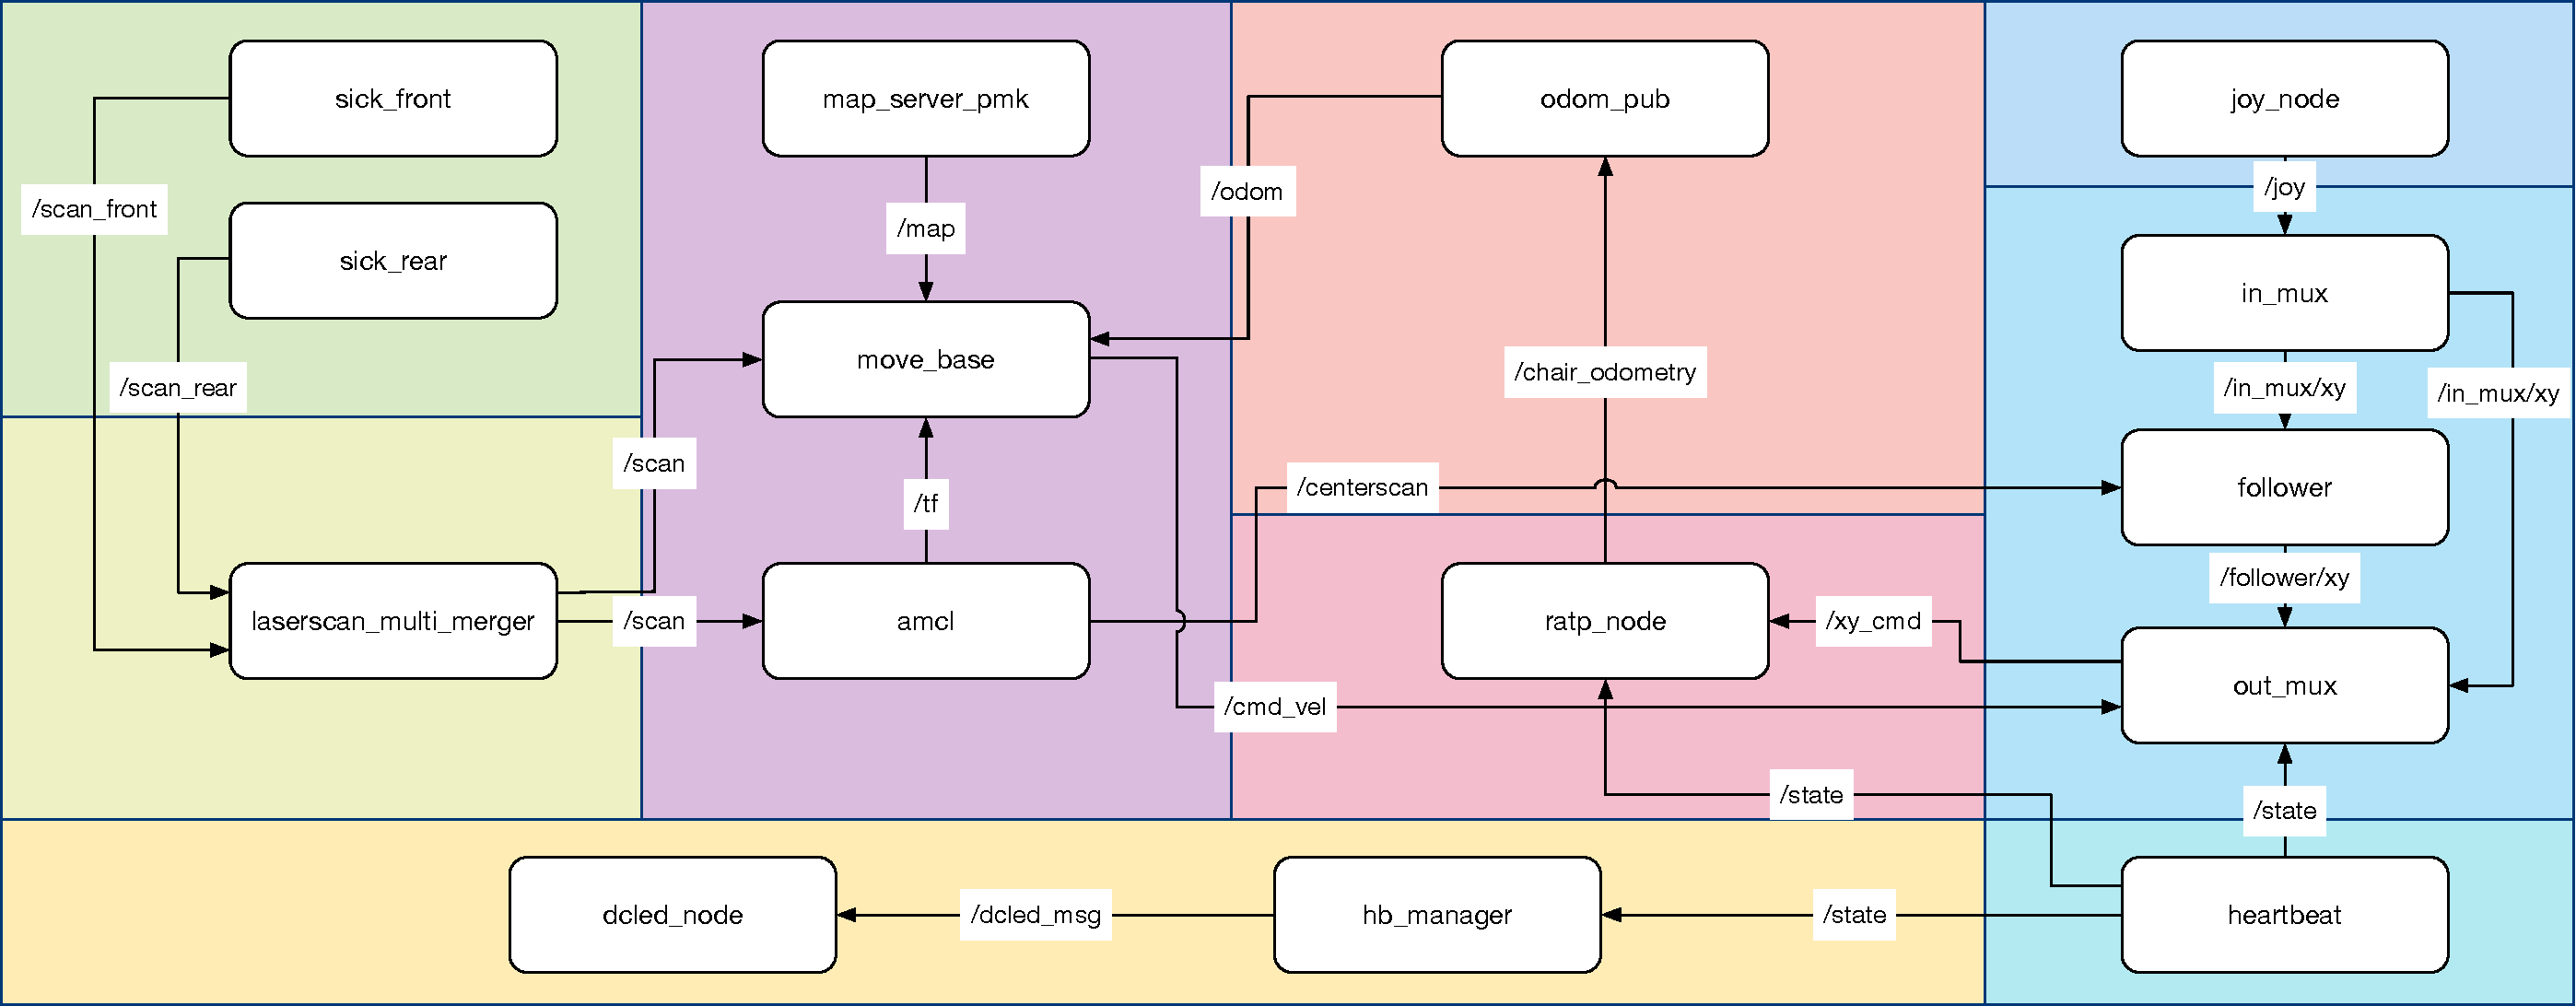
\includegraphics[width=0.95\textheight]{gfx/pmk/softwarearchitecture}
	\caption{Original design of the architecture of the autonomous wheelchair.}
	\label{fig:pmk-doc}
	\end{figure}
\end{landscape}

\begin{landscape}
	\begin{figure}[t]
	\centering
	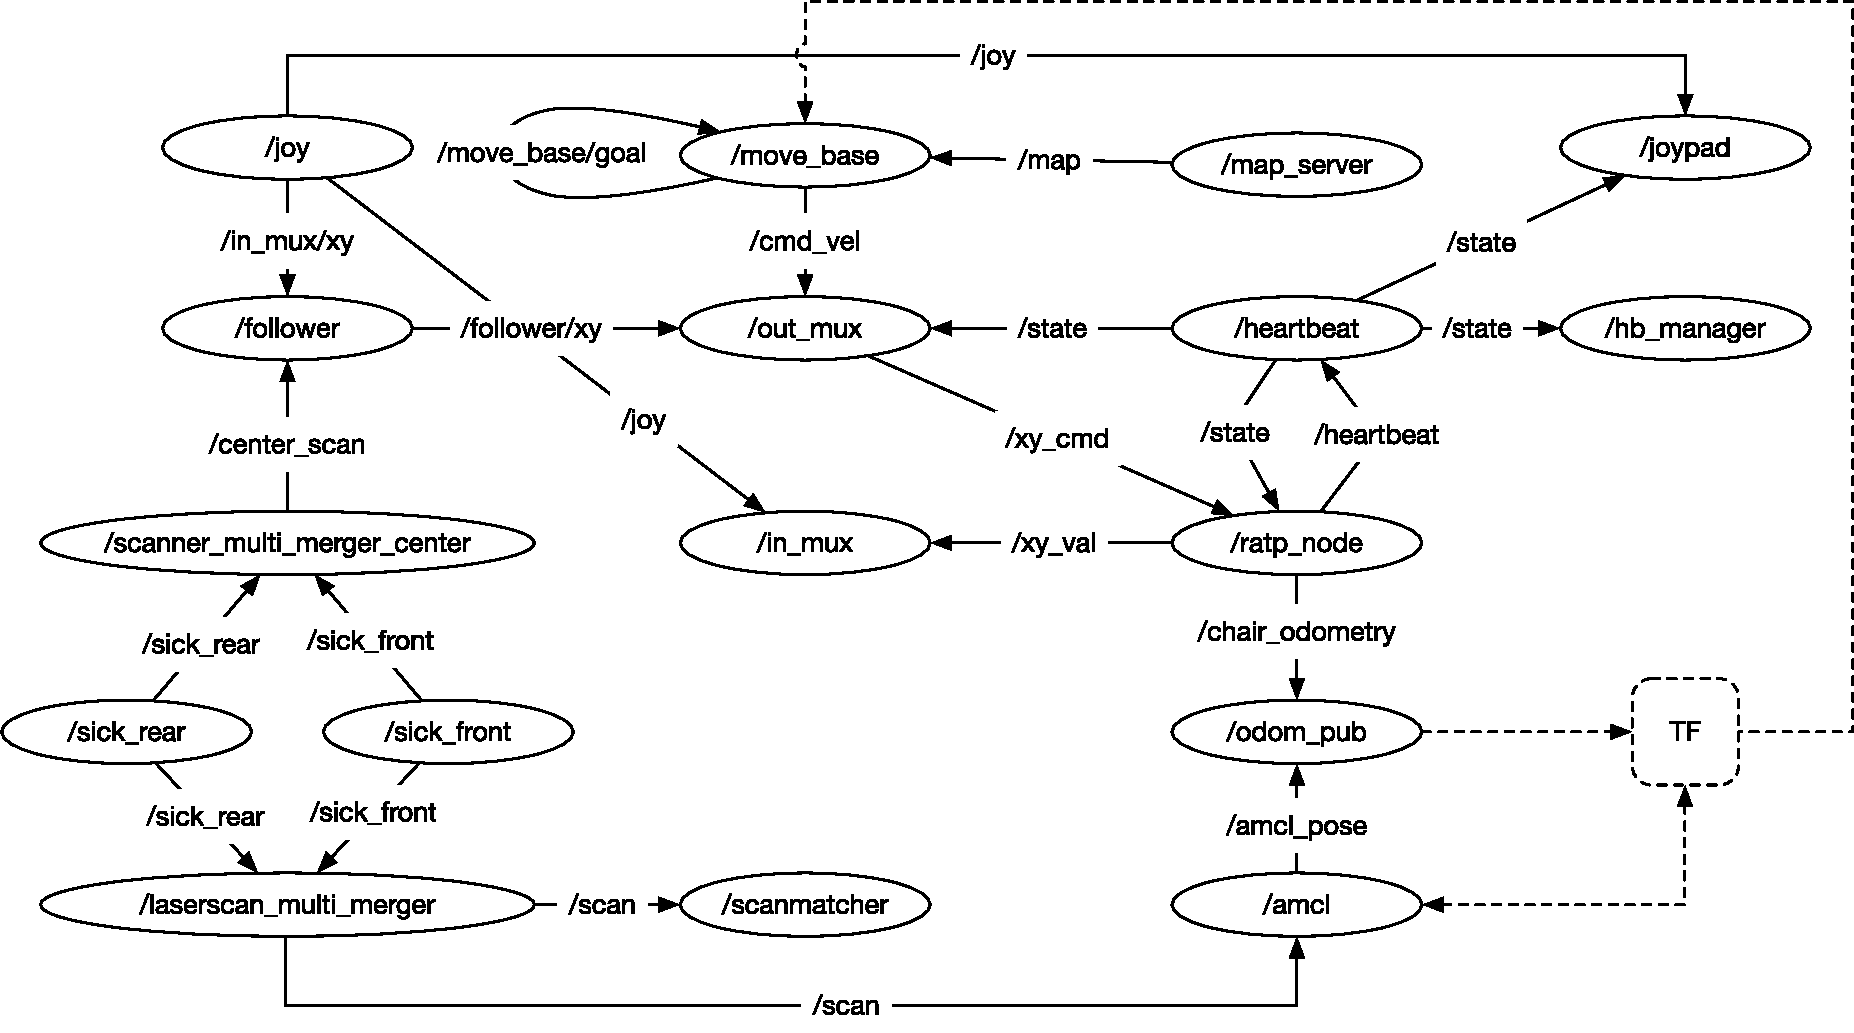
\includegraphics[width=0.95\textheight]{gfx/pmk/hand-graph}
	\caption{Runtime ROS graph of the hand-written architecture.}
	\label{fig:pmk-graph}
	\end{figure}
\end{landscape}

\begin{landscape}
	\begin{figure}[t]
	\centering
	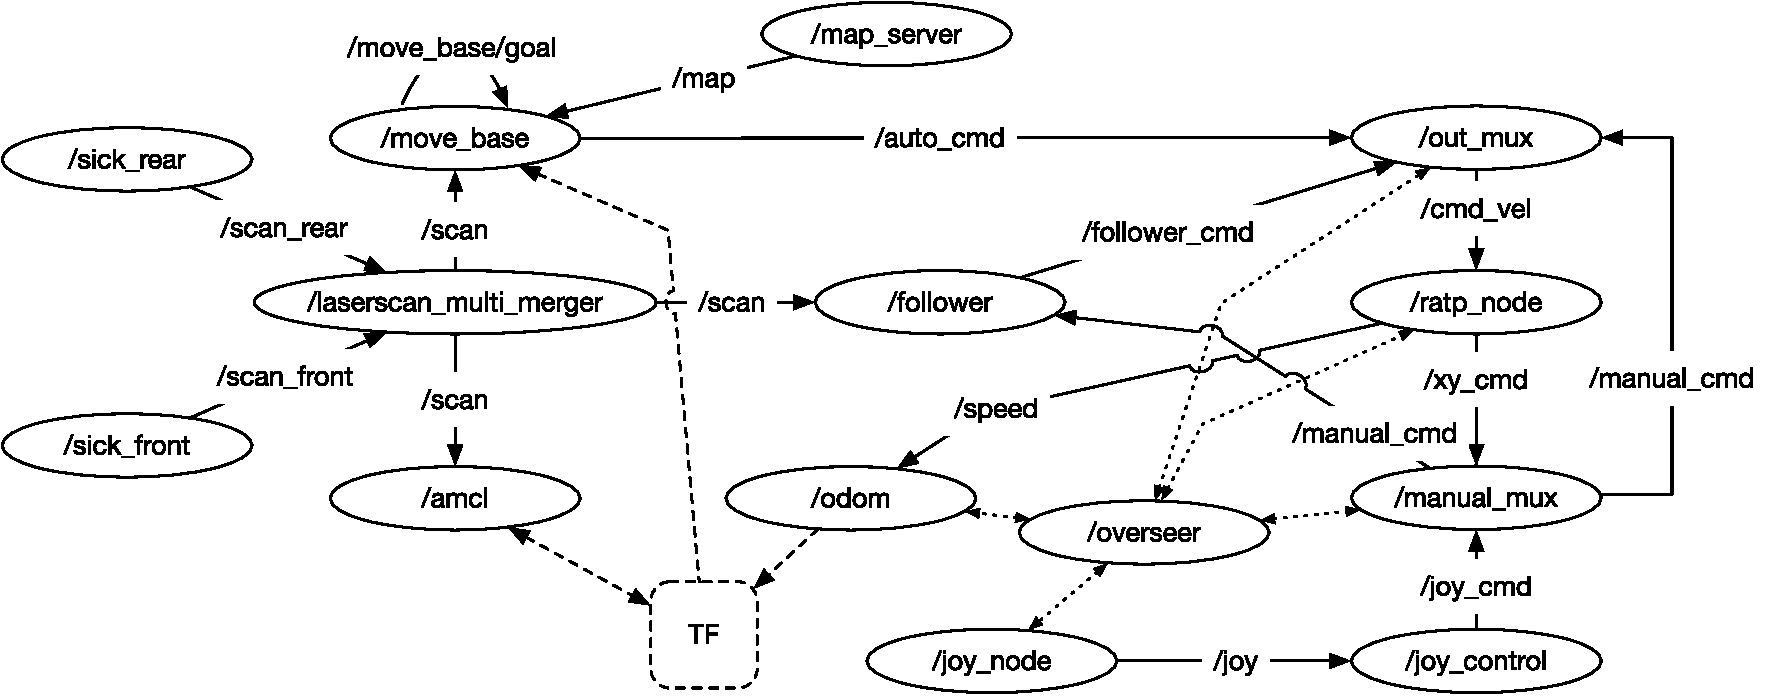
\includegraphics[width=0.95\textheight]{gfx/pmk/gen-graph}
	\caption{Runtime ROS graph of the automatically generated architecture.}
	\label{fig:gen-graph}
	\end{figure}
\end{landscape}

\begin{figure}[t]
\centering
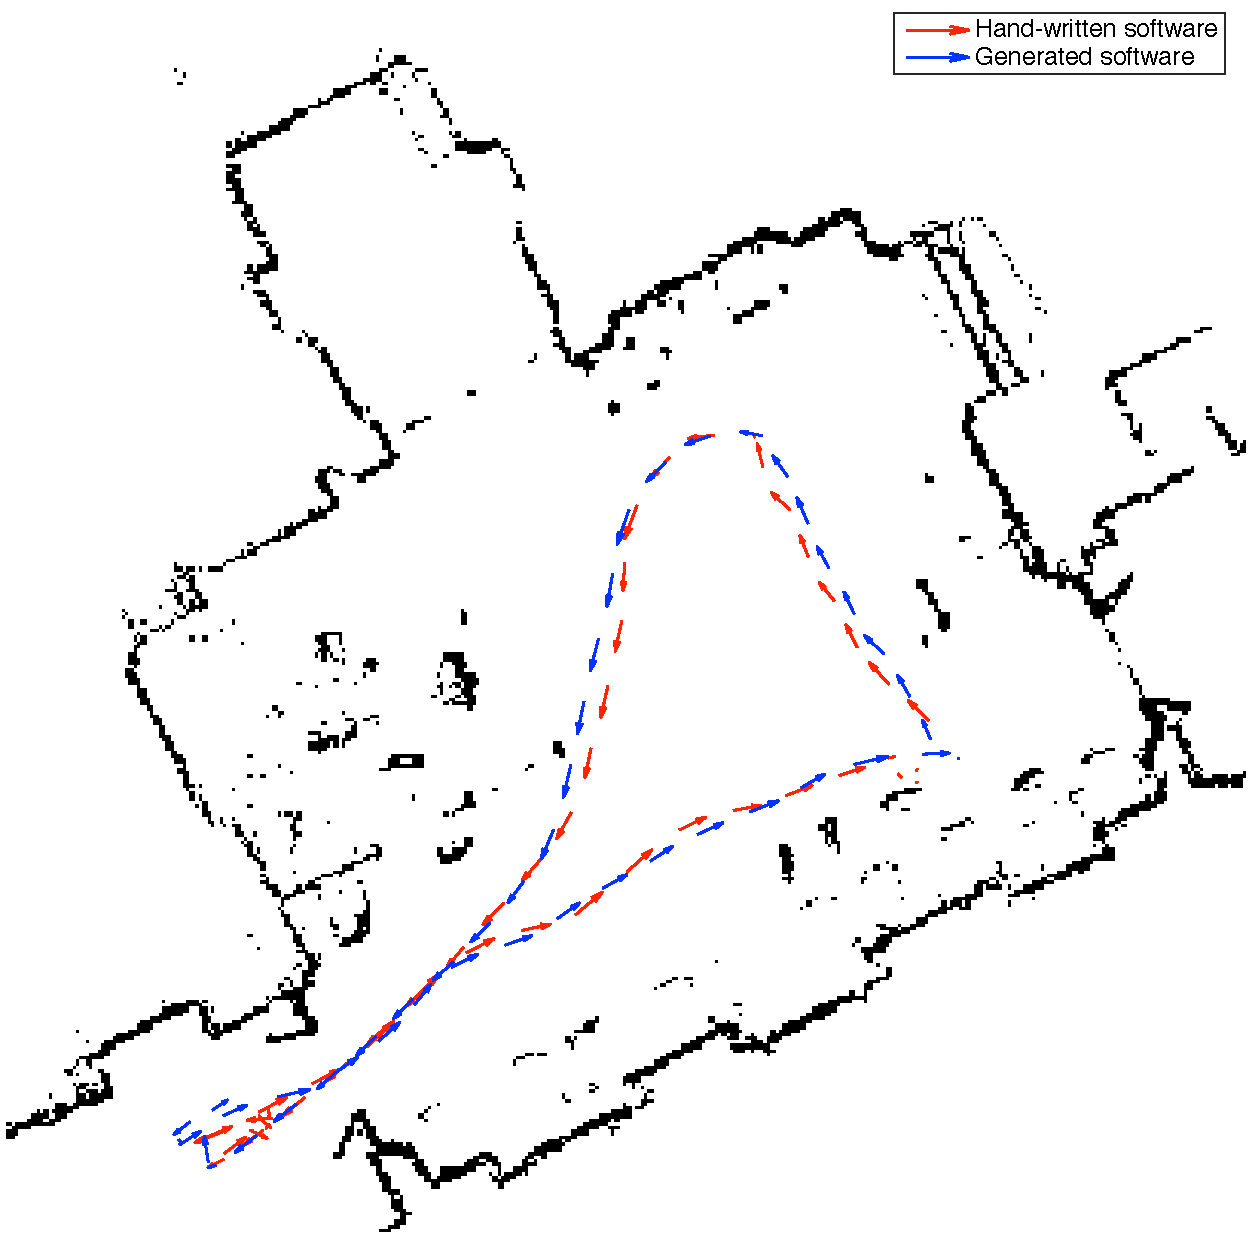
\includegraphics[width=0.95\textwidth]{gfx/pmk/path-followed}
\caption[Trajectory comparison.]{Comparison between the trajectory followed by the robot equipped with the hand-written software (in red) and the automatically generated implementation (in blue).}
\label{fig:path}
\end{figure}

\subsection{Comparison}
The aim of this use case was to showcase how a complete and functional architecture can be designed and developed entirely using a model-based approach combined with automatic code generation. Starting from an existing architecture was useful for multiple reasons: clear use case and requirements for the robot, existing implementations for all the problem-specific features, precise target functionalities, reference benchmark for the behaviour of the autonomous wheelchair. It was important for us to be able to compare the result of our approach to an existing implementation. In this section, we will analyse the original architecture to show the similarities with the automatic generated one and also to highlight existing problems that were solved using a model-based design approach.

First of all, we have to compare the design of the architecture of the wheelchair according to the documentation (Figure~\ref{fig:pmk-doc}) with the runtime computation graph generated by ROS (Figure~\ref{fig:pmk-graph}). With a quick analysis it is possible to see that they do not match. Some nodes mentioned in the documentation are not present in the graph (\eg, \textit{dcled\_node}) or vice versa (\eg, \textit{scanner\_multi\_merger\_center}), while others have been replaced (\eg, the standard \textit{map\_server} in place of the custom \textit{map\_server\_pmk}). This is not surprising, the PMK is an ongoing research project where multiple people with varying experience contributed to it. As a result, features were added directly to the codebase without propagating them in the documentation or in the original design. As the project progressed, some of the features were removed, but they left some dangling dependencies behind, in the form of design choices and components. This problem is exacerbated by the fact that ROS does not provide any tool to visualise and analyse the complete architecture before runtime. The only way is to run the entire system and then view the ROS graph using tools like \textit{rqt\_graph}. However, even this approach is limited, since it only shows topics, but no services or actions. Of course, a model-based approach does not automatically solve all these problems, since a developer can, and sometimes needs to, directly modify the codebase. However, by combining the models with the automatic code generation we can create an environment where good practices and designs are encouraged and more natural.

With a deeper analysis of the runtime graph it is possible to identify some architectural problems, that were not present in the original design but were introduced in sequential iterations of the project. There are three fundamental issues that could cause unexpected behaviours of the robot.
\begin{itemize}
\item There is a circular dependency between \textit{odom\_pub} and \textit{amcl}. Both nodes are in charge of estimating the position of the robot. The former uses velocity measurement coming from the wheelchair, while the latter matches laser rangefinder data with a know map. The circular dependency happens because each of them expect from the other an initial position to start the estimate. Given how the two algorithms are implemented, an incorrect starting position would not compromise the correct functioning of the system, however it may cause unexpected behaviour, especially after the initial start up of the system.
\item The odometry is estimated twice in the system. This is not directly visible from the graph presented in Figure~\ref{fig:pmk-graph}, since it is not detailed enough, however, the \textit{rapt\_node} pre-compute the odometry of the platform and provide it, together with the velocity measurements, to \textit{odom\_pub}. The initial computation is then discarded and recalculated again directly from the velocity. While this causes no malfunction, it is not a consistent design choice to perform a specific processing twice in the same architecture. 
\item The management of the laser scanner measurements is flawed in multiple ways. As explained in Section~\ref{sec:pmk-model}, the navigation subsystem requires an unified source of laser information. In the original documentation, there was a single node in charge of merging the two laser sources, however, in the actual architecture, there are two nodes with the same task: \textit{scanner\_multi\_merger\_center} and \textit{laserscan\_multi\_merger}. Moreover, it is not visible from the computation graph, but the lunch file of the original architecture included a third laser scan merger node,  which is killed at start up since it has the exact same name of another one, and ROS forbids it. Finally, there is a \textit{scanmatcher} node that subscribes to a topic but has no role in the architecture, a leftover dependency from a removed functionality. Since the duplicated nodes are functionally identical, the overall functionalities of the architecture are preserved. However, such a configuration is a waste of computational power and a potential source of significant and dangerous inconsistencies.
\end{itemize}

For comparison, Figure~\ref{fig:gen-graph} shows the runtime graph of the architecture resulting from the model-based design and automatic code generation. The overall structure of the system is very similar to the original architecture. However, all the issues identified before have been solved.
\begin{itemize}
\item There is no circular dependency between \textit{amcl} and \textit{odom}. They receive the initial position independently as a parameter or through an external topic.
\item The odometry is estimated only once in the \textit{odom} node. The \textit{ratp\_node} provides directly and only the current speed of the wheelchair as a \textit{Twist} message.
\item Only one node is in charge of unifying the laser sources and the \textit{scanmatcher} node has been removed.
\end{itemize}

Analysing the ROS graph is useful to provide an overview of the quality of the design of the architecture, however, it gives no insight on the actual functionalities of the system. As seen from the original architecture, design flaws do not always translate in a compromised system or in faulty behaviours. The robotic wheelchair equipped with the handcrafted architecture supported full autonomous driving with no serious issues, except for minor problems caused by an unstable communication with the low-level control module. This means that we can use the behaviour of the original architecture  to provide an empirical proof of the correctness of the generated architecture. We performed a comparison between the path followed by the wheelchair when running the original system in autonomous mode, and then we gave the same goal to the generated architecture. Figure~\ref{fig:path} shows the result. The resulting paths are extremely similar, indicating that not only the generated architecture replicates the same results of the original one, but also that all the problem-specific implementations have maintained their original functionalities even after being transposed in the automatically generated ROS environment.

\begin{figure}[t]
    \centering
    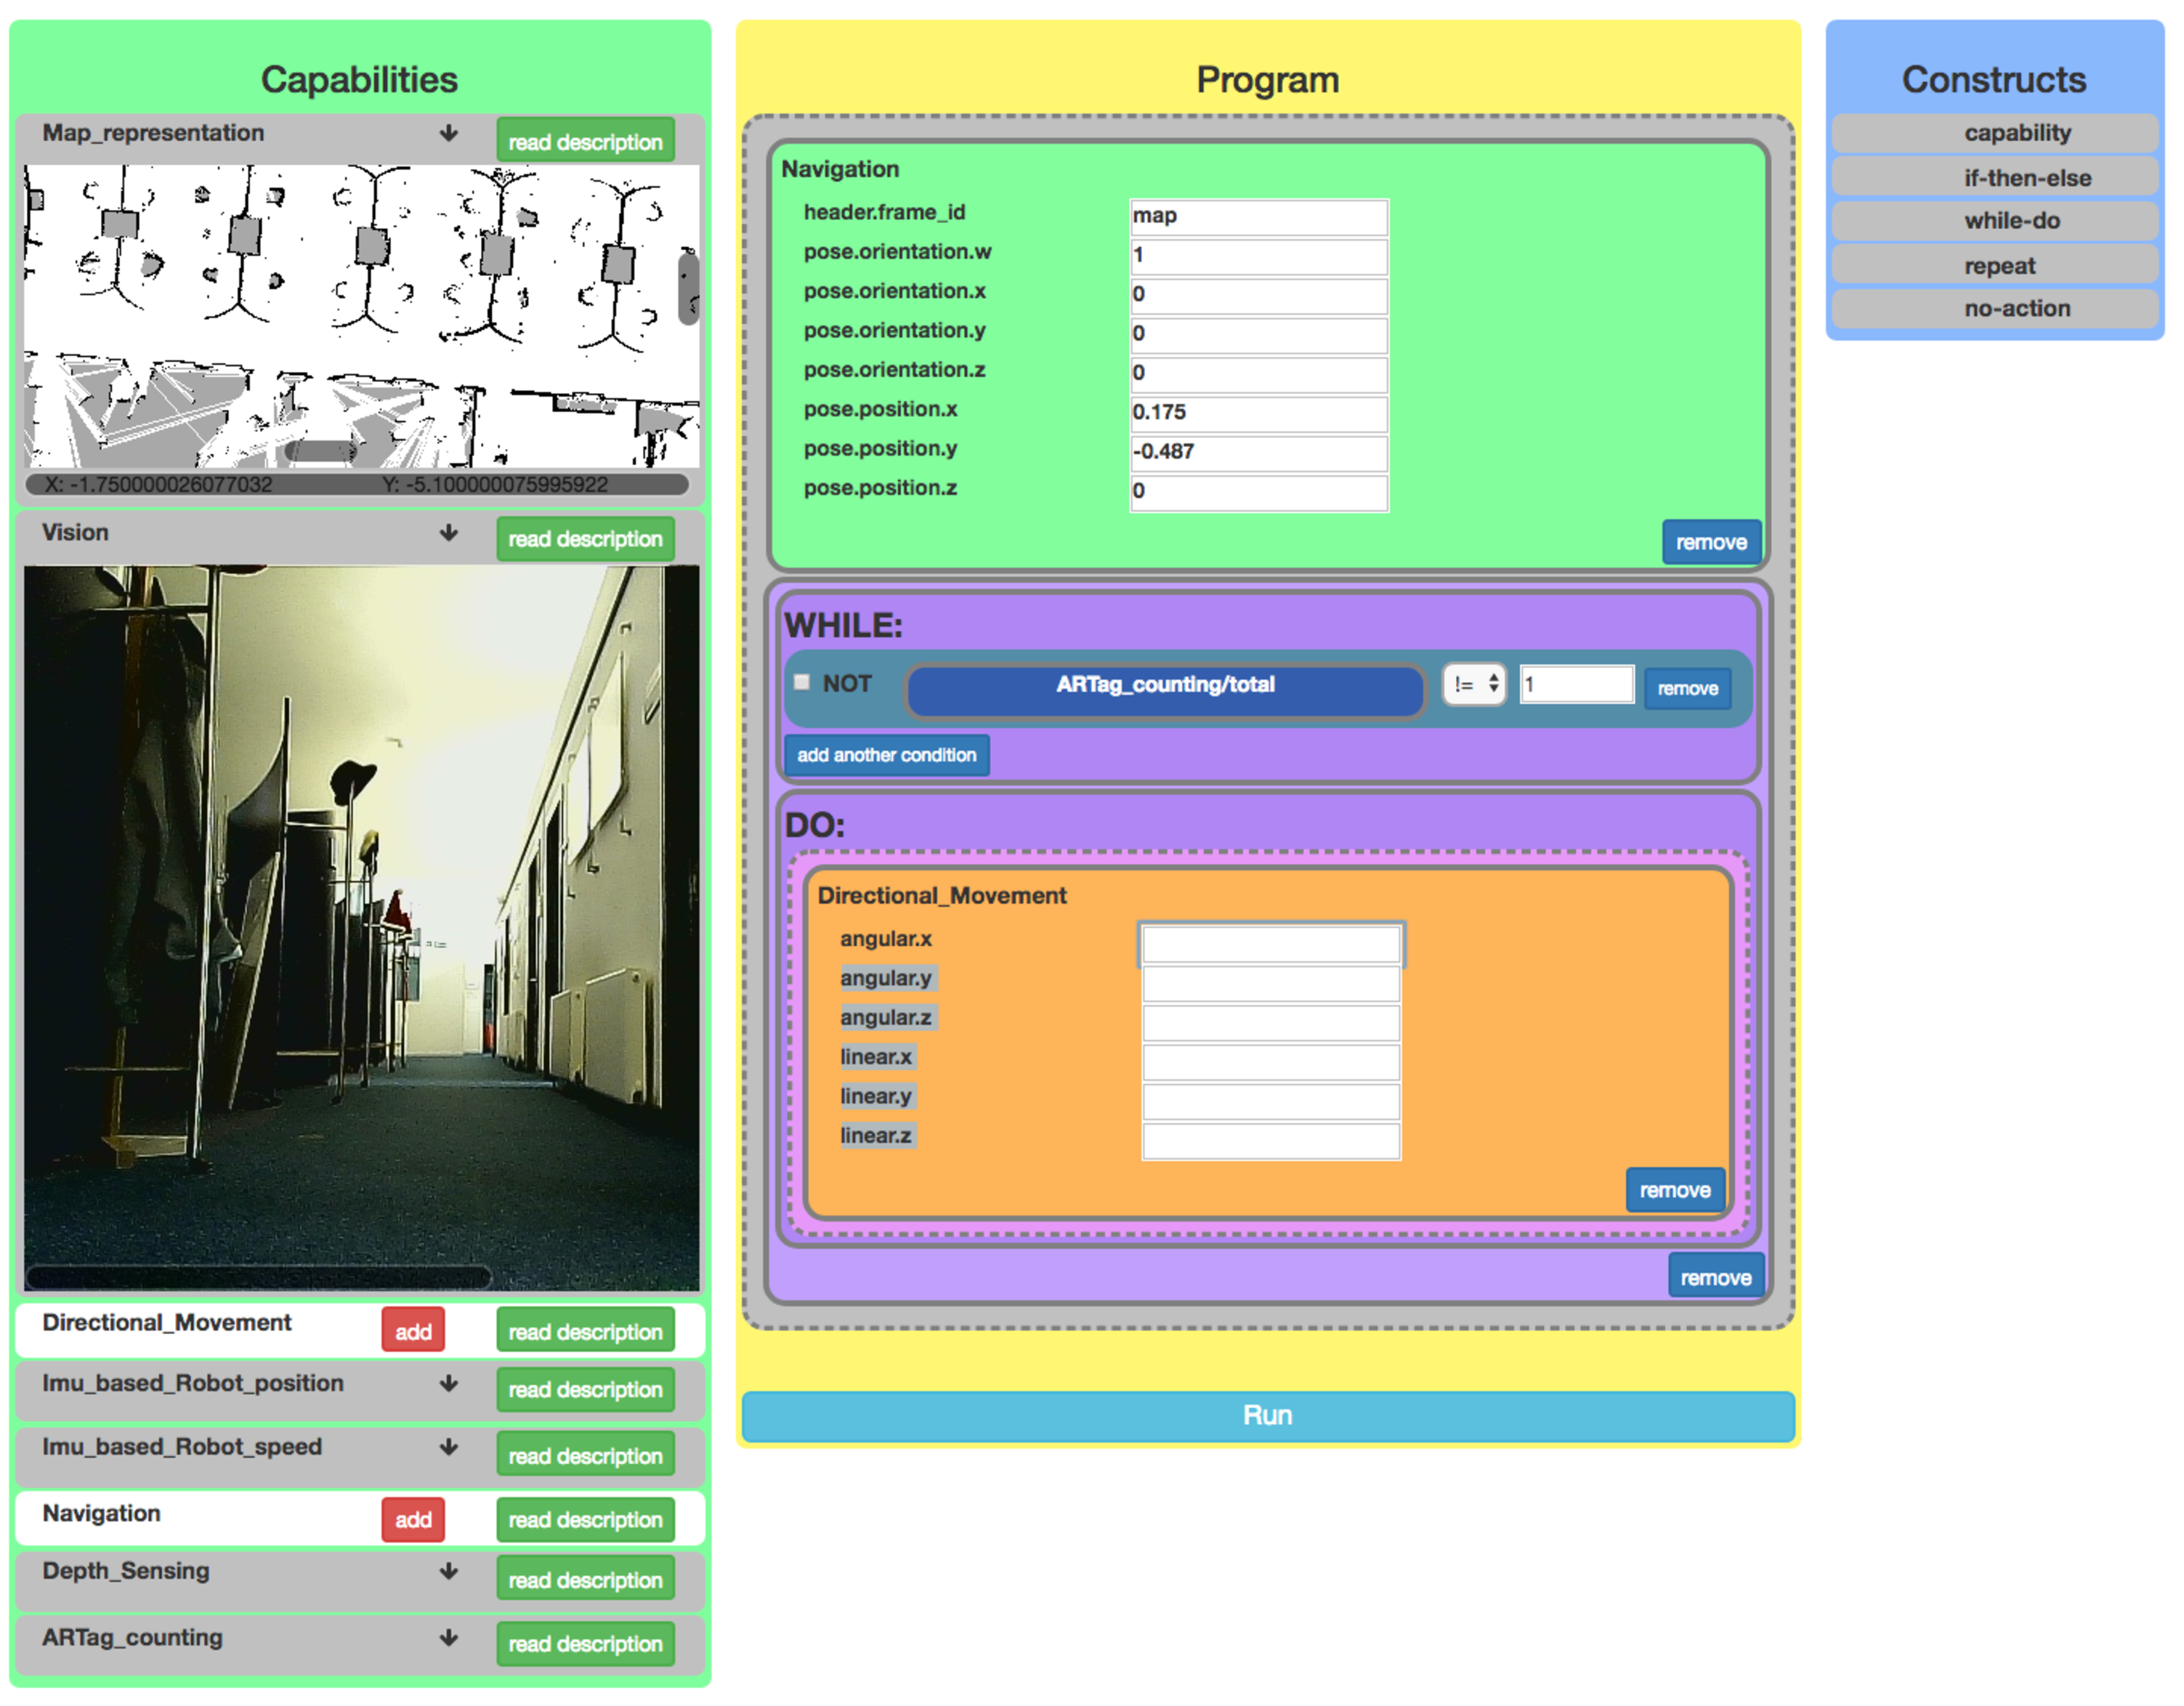
\includegraphics[width=0.9\textwidth]{gfx/onto/web}
    \caption{The web interface used to interact with the capabilities evoked by the robot.}\label{fig:web-api}
\end{figure}

\section{Web interface}
By decoupling the \textit{Server} from the \textit{OntoRob Interface} we can create multiple interfaces that can access the functionalities of the robot through the capability system. In an effort to explore different approaches, push the boundaries of our implementation, and test it directly with users in a controlled environment, we developed an additional \textit{Web Interface}. An instance of this interface is visible in Figure~\ref{fig:web-api}. It replaces the \textit{OntoRob interface} and interacts directly with the \textit{Server}.

Once set up, the interface is accessible from any web browser, it was specifically designed to be simple, intuitive, easy to understand, and accessible. The aim is not to implement a complete interface to program and remotely control a robot, but to create a proof-of-concept that can be used to inspect the status of the robot (through \textit{read}-capabilities) and give a sequence of simple command (through \textit{write}-capabilities). To make the interface more complete, we implemented a simple programming language to chain multiple commands together and use conditional statement based on the output of \textit{read}-capabilities.

In this section, we give a description of the graphical user interface presented by the \textit{Web interface}, then we show the results obtained in an experiment where a set of user with no previous experience in robotics or ROS had to develop programs using the interface to complete  a simple robotic task with two different platforms.

\subsection{GUI description}
The \textit{Web interface} is designed to be essential and to show as much information as possible without overloading the user. It is divided in three different panels, each one focusing on a specific aspect of our approach: the capability panel, it presents the functionality of the robot in a compact way, the program panel, it is the main part of the interface and it contains the program created by the user, and construct panel, it is the ``toolbox'' the user has to create the program.

\paragraph{Capability Panel} This panel presents the capabilities abstracted by the combined work of the \textit{Analyzer} and the \textit{Server}. When activated, the \textit{Web interface} contacts the \textit{Server} and retrieve the list of all the currently active and accessible capabilities. The retrieved list is presented to the user in various forms depending on the nature of each capability. First of all, the distinction between \textit{read}-capabilities and \textit{write}-capabilities. The former represent the flow of information coming from the robot to the user, therefore their value is constantly updated and visualised in the GUI. For example, the box connected to the \textit{Robot position} capabilities contains three fields (\ie, x, y and z coordinates) showing the current position of the robot in space, the \textit{Web Interface} periodically queries the \textit{server} to update the content of the fields with the most recent position. The latter represent the entry points a user can exploit to interact with the robot, therefore they are presented only as a list of available capabilities. For each capability the most suitable visualisation system is used. For instance, the velocity of the robot is more understandable in numerical form showing the raw content of the original ROS message, while the video feed of the on-board camera is better if rendered to show the actual pictures. Each capability is associated with a description to help the user understand the information provided, and exploit the entry point to interact with the robot.

\paragraph{Program Panel} The central area of the \textit{Web interface}, as seen in Figure~\ref{fig:web-api}, is dedicated to the user to create a program to send to the robot. The user can select each sub-panel of the programming area to interact with it. By selecting the outermost panel (\ie, the grey border around the whole program in the figure) the user can add a new capability or a new programming paradigm, while by selecting internal panels (\eg, the pink border in the \texttt{DO} panel) the user can define subroutines and specify conditions. When added to the \textit{Program panel}, a capability will show the available parameters as fillable fields, so the user can specify the actual value to send to the robot. Once the user is satisfied with the set of commands, he can send them to the robot using the \textit{Run} button. When the button is pressed, the commands are converted by the \textit{Web interface} in a JSON file and sent to the \textit{Server}. The \textit{Server} decode the list of instructions and execute them in the necessary order through the \textit{Dynamic node}.

\paragraph{Construct Panel} The rightmost panel of the \textit{Web interface} represents the ``toolbox'' of the user. We did not want to implement a complex and fully functional programming language, therefore we focused on the most essential construct to give the user enough freedom. The first on the list is the capability: by using this construct the user can add a special container to the program, then, by selecting the container, add a specific \textit{write}-capability by using the \textit{add} button from the \textit{capability panel}. Then there are all the constructs available to change the control flow of the program: \textit{if-then-else}, for a conditional jump, \textit{while-do}, for a condition-based loop, and \textit{repeat}, to repeat a set of instructions a specific amount of times. A program can be created as an imperative programming language, in which the atomic blocks are either invocations of the available robot capabilities, or any conditional operator. An additional \textit{no-action} construct can be used to perform a no operation (\eg, an \textit{if-then-else} with an empty \textit{else} statement), or to create waiting loops. The parameters of a capability can be used in the conditions, to exploit any robot output and drive the program flow (\eg, moving forward until an object is detected). 

\subsection{Experimental Setup}
 Each user was asked to perform four exercises of increasing difficulty. These corresponded to creating a program allowing a robot to achieve a specific task. In order to demonstrate that the ontology-based system could allow the abstraction of robot capabilities independently from the platform, we set up two variants of each exercise, a simulated one with a ground wheeled robot operating in an office environment (\texttt{s}-variant), and a real-world one with a drone flying in an indoor space (\texttt{r}-variant). Table~\ref{tab:setting} presents the robot capabilities available in each setting.

\begin{table}
    \myfloatalign
    \begin{tabularx}{\textwidth}{l X X} \toprule
\tableheadline{Mode} &\tableheadline{\texttt{s}-variant} &\tableheadline{\texttt{r}-variant} \\ \midrule
 & \multirow{2}{*}{autonomous navigation} & take-off  \\
write &\multirow{2}{*}{directional movement}& land \\
& &  directional movement \\ \midrule
 & vision &  \\ 
 & current position & vision\\
read & current speed  & current position  \\
 & map representation & object recognition\\
 & object recognition \\
\bottomrule
    \end{tabularx}
    \caption[Robot capabilities for the two exercise variants.]{Robot capabilities for the two exercise variants.}  \label{tab:setting}
\end{table}

\paragraph{Exercise~1: Single command} The first exercise  requires the user to send a single command to the robot (\ie, exploit a single \textit{write}-capability). The exercise was designed to let the user familiarise with \textit{Web interface} by focusing only on understanding the concept of capability and how to use them to operate the robot. In the \texttt{s}-variant, the user needs to exploit two capabilities: \textit{Map representation} to understand the current position of the robot and select a potential destination, and \textit{Autonomous navigation} to command the robot  to reach the specified destination. For the \texttt{r}-variant, the exercises starts when the drone already performed a successful take-off (\ie, the drone is already flying), therefore the user needs to use only the \textit{Directional movement} capability to move the drone in any direction.

\paragraph{Exercise~2: Command sequence} The second exercise requires the user to chain together a list of commands to send to the robot (\ie, exploit multiple \textit{write}-capabilities or the same one multiple times). The objective of this exercise is to let the user know that he can create a complex behaviour for the robot, and not only send atomic actions. The \texttt{s}-variant is a direct extension of the previous exercise, since the user needs to instruct the robot to navigate to two different locations, one after the other. In the \texttt{r}-variant, the exercise will start again with a drone that has successfully performed a take-off, the user has to instruct the drone with any motion command, then command the drone to land using the \textit{Land} capability. 

\paragraph{Exercise~3: Condition-based halt} The third exercise requires user to implement a sequence of actions with a termination condition (\ie, use a condition to manage the execution of a \textit{write}-capability). In this exercise we introduce the first conditional constructs (\eg, \textit{repeat} and \textit{while-do}) to the user, and we let him discover that he can create complex programs. In the \texttt{s}-variant, the robot needs to patrol three different locations, stopping only once all the locations had been visited at least twice. This requires to exploit the \textit{Autonomous navigation} capability and to use the \textit{repeat} construct. In the \texttt{r}-variant, the user has to instruct the drone to keep spinning until it has performed at least a ration of \ang{180} on itself, at which point the drone will have to land. In this case the user has to exploit both \textit{write}-capabilities to pilot the drone (\ie, \textit{Directional movement} and \textit{Land}) and a \textit{read}-capability (\ie, \textit{Robot orientation}) together with a conditional statement, in order to complete the exercise.

\paragraph{Exercise~4: Object recognition} In the final exercise, the user had to combine base capabilities (\eg, \textit{Directional movement} or \textit{Navigation}) with advanced capabilities based on additional functionalities introduced in the robot. In particular, the user had to create a behaviour for the robot based on the detection of ARtags. The aim of this exercise is to show to the user that it is possible to extend the functionalities of the robot with extra capabilities and to increase the complexity of the program. In the \texttt{s}-variant, the robot had to patrol a set of locations until an ARtag is detected. In the \texttt{r}-variant, the user had to implement three different movement behaviours for the drone each of them triggered by a different ARTag.

\subsection{Results and discussion}

A total of fourteen users were involved in the evaluation, equally shared between the \texttt{s}- and the \texttt{r}-variant. All the users had at least some basic programming knowledge, however, none of them had any robotic background or any previous experience with ROS or other robotic middleware or framework. As a starting point, users were first allowed to familiarise themselves with the interface, namely through clicking on the different sections to understand the general behaviour of the tool. To make the task of resolving the different exercises more challenging for the users, they were prevented from reading the description of the capabilities in this initial familiarisation phase. After this first step, they were  asked to solve all four exercises one after the other. For every exercise, we measured the time from the end of the task description until the final execution of the program.

\begin{table}
\myfloatalign
\newcolumntype{C}{>{\centering}X}%
\begin{tabularx}{\textwidth}{l C C C C} \toprule
 & Ex. 1 & Ex. 2 & Ex. 3 & Ex. 4 \tabularnewline \midrule
\multicolumn{5}{c}{\texttt{s}-variant} \tabularnewline \midrule
$\overline{pb}$ & 1 & 2 & 4 & 9.5   \tabularnewline
no. cap & 1     & 1     & 1     & 2     \tabularnewline
$\overline{t}$ & \makecell{1:22 \\ $\pm$ 42s} & \makecell{1:04 \\ $\pm$ 23s} & \makecell{1:15 \\ $\pm$ 16s} & \makecell{6:52 \\ $\pm$ 1:46} \tabularnewline
\midrule
\multicolumn{5}{c}{\texttt{r}-variant} \tabularnewline \midrule
$\overline{pb}$ & 1     & 2     & 4     & 8 \tabularnewline
no. cap  & 1     & 2     & 4     & 4 \tabularnewline
$\overline{t}$ & \makecell{1:16 \\ $\pm$ 3s} & \makecell{01:16 \\ $\pm$ 8s} & \makecell{4:05 \\ $\pm$ 15s} & \makecell{5:47 \\ $\pm$ 1:39} \tabularnewline
\bottomrule
\end{tabularx}
\caption{Results obtained by the non-experts for the \texttt{s}-variant and the \texttt{r}-variant.}
\label{tab:results-users}
\end{table}

Table~\ref{tab:results-users} shows the average time ($\overline{t}$) required by the users to solve each exercise, along with the average number of programming blocks ($\overline{pb}$) and the number of capabilities (\textit{no. cap}) required to solve the task. All the exercises were successfully carried out by all users. As one can see, Ex.~1 took slightly longer (especially in the \texttt{s}-variant), when compared with other more complex exercises. This can be attributed to the time users required to familiarise themselves with the capabilities of the robot they were working with, which they did not know beforehand. The relatively high variance in the time taken for Ex.~4 is due to this particular exercise having multiple solutions, some of which taking longer to implement than others. 

A key, straightforward conclusion from this table is that users of this tool, who had no experience of programming robots and no prior knowledge of the architecture of the robot they were manipulating, managed to successfully program such a robot to achieve tasks from the very simple Ex.~1 to the more difficult Ex.~4 in a matter of a few minutes. Considering the inherent complexity of robot programming and of understanding not only what a robot can do (what capabilities it possesses), but also how to use it (how to invoke those capabilities), this can be considered a non-trivial achievement. 

A direct comparison with how the same users would have achieved the same tasks without the tool provided is not feasible and would turn out to be meaningless. However, given that those users are not familiar with ROS,  the process of identifying the different components of the robot, what they do, and how to use them, would require more than the few minutes required with our interface. ROS is a complex framework, requiring hours of practice to master. In addition, analysing the runtime graph of the specific robot to understand which topics and services are being used (\ie, what the tool does through the ontology) is far from an easy task. A number of ROS nodes would need to be implemented from scratch to encapsulate the required functionalities, and manage the correct publishers and subscribers. Lastly, the nodes would need to be deployed and integrated with the robot architecture. Knowledge of the specific packages (\eg, \textit{move\_base} for autonomous navigation) is also required by some of the exercises. In other words, while a direct comparison could not have been performed, achieving the same results with ROS would have undoubtedly required a significantly higher effort by our non-expert users compared to our tool.

\begin{table}
\myfloatalign
\newcolumntype{C}{>{\centering}X}%
\begin{tabularx}{\textwidth}{l C C C C} \toprule
& Ex. 1 & Ex. 2 & Ex. 3 & Ex. 4 \tabularnewline \midrule
\multicolumn{5}{c}{\texttt{s}-variant} \tabularnewline \midrule
LOC & 35 & 58 & 64 & 82 \tabularnewline
no. com & 1 & 2 & 2 & 3 \tabularnewline
no. msg & 1 & 2 & 2 & 3 \tabularnewline
\midrule
\multicolumn{5}{c}{\texttt{r}-variant} \tabularnewline \midrule
LOC & 34 & 39 & 56 & 59 \tabularnewline
no. com & 1 & 2 & 4 & 4 \tabularnewline
no. msg  & 1 & 2 & 3 & 3 \tabularnewline
\bottomrule
\end{tabularx}
\caption{Results obtained by the expert for the \texttt{s}-variant and the \texttt{r}-variant.}
\label{tab:results-expert}
\end{table}

As an additional point towards the validity of our claim that our tool reduces the effort required to exploit robots' capabilities and therefore make them more accessible, we asked an expert in robotics with extensive experience in ROS to achieve the same task. Once again, the objective here is not to compare the experts to the non-experts using two different frameworks, but to provide an intuitive understanding of the difficulty of realizing the tasks achieved by our users without our tool. In Table~\ref{tab:results-expert}, we therefore show for each task in each variant:
\begin{itemize}
\item the number of lines of code used by the ROS expert (\textit{LOC}), 
\item the number of ROS communication components (publishers and subscribers) employed (\textit{no. com}),
\item the number of message types used (\textit{no. msg}). 
\end{itemize}

These metrics give an estimate of the effort required by a ROS developer to solve the specified tasks. Lines of code set a lower bound for the implementation time, while the number of components and messages outline the complexity of the solution.

This comparison further shows how programming a robot is made ``easier'' and, through abstracting capabilities from the technical aspects of their implementation, requires less complexity. Our approach and the associated tool therefore represent a viable solution to enable non-expert users to exploit robots in ways that were before only accessible to expert ROS programmers. 

%*****************************************
